\documentclass[11pt,a4paper,twocolumn]{article}
\usepackage[utf8]{inputenc}
\usepackage[T1]{fontenc}
\usepackage{lmodern}
\usepackage{amsmath,amssymb,amsfonts,amsthm}
\usepackage{mathtools}
\usepackage{geometry}
\usepackage{booktabs}
\usepackage{array}
\usepackage{graphicx}
\usepackage{xcolor}
\usepackage{listings}
\usepackage{tikz}
\usetikzlibrary{arrows.meta, positioning}
\usepackage{hyperref}
\usepackage{fancyhdr}
\usepackage{titlesec}

\geometry{top=2.0cm, bottom=2.2cm, left=1.6cm, right=1.6cm, columnsep=0.7cm}

\definecolor{darkblue}{RGB}{15, 45, 95}
\definecolor{codebg}{RGB}{246, 248, 250}
\definecolor{codeframe}{RGB}{210, 215, 222}

\hypersetup{
    colorlinks=true,
    linkcolor=darkblue,
    urlcolor=darkblue,
    citecolor=darkblue
}

\lstset{
    backgroundcolor=\color{codebg},
    frame=single,
    rulecolor=\color{codeframe},
    basicstyle=\ttfamily\footnotesize,
    breaklines=true,
    captionpos=b,
    keepspaces=true,
    showspaces=false,
    showstringspaces=false,
    showtabs=false
}

\tikzset{
    meter/.style={
        draw,
        fill=codebg,
        minimum width=0.52cm,
        minimum height=0.42cm,
        inner sep=0pt,
        path picture={
            \draw[thin] ([yshift=-2pt]path picture bounding box.center) ++(-0.16cm, 0) arc (180:0:0.16cm);
            \draw[-{Latex[length=2.2pt]}, thin] ([yshift=-2pt]path picture bounding box.center) -- ++(0.11cm, 0.19cm);
        }
    },
    gate/.style={
        draw,
        fill=white,
        minimum size=0.42cm,
        inner sep=1pt,
        font=\small
    },
    smallgate/.style={
        draw,
        fill=white,
        minimum width=0.38cm,
        minimum height=0.42cm,
        inner sep=0pt,
        font=\scriptsize
    },
    target/.style={
        circle,
        draw,
        inner sep=0pt,
        minimum size=3.2mm,
        path picture={
            \draw[thin] (path picture bounding box.north) -- (path picture bounding box.south)
                        (path picture bounding box.west) -- (path picture bounding box.east);
        }
    },
    control/.style={
        circle,
        fill=black,
        inner sep=0pt,
        minimum size=1.7mm
    }
}

\pagestyle{fancy}
\fancyhf{}
\fancyhead[L]{\footnotesize Compiling Shor's Algorithm in \texttt{|BF>} (Bra-Ket-Fuck)}
\fancyhead[R]{\footnotesize Technical Report $\cdot$ Architecture Specification v1.1 $\cdot$ October 2026}
\fancyfoot[C]{\footnotesize \thepage}

\newcommand{\bra}[1]{\langle #1 |}
\newcommand{\ket}[1]{| #1 \rangle}
\newcommand{\braket}[2]{\langle #1 | #2 \rangle}
\newcommand{\ketbra}[2]{| #1 \rangle\langle #2 |}
\newtheorem{theorem}{Theorem}
\newtheorem{lemma}{Lemma}

\title{\vspace{-0.5cm}\textbf{\Large Compiling Shor's Algorithm to the Dirac--M\"uller Quantum Tape:\protect\\ Linear Nearest-Neighbor Modular Exponentiation and\protect\\ Semiclassical Qubit Recycling in \texttt{|BF>}}}
\author{\large mat-ocl (\href{https://github.com/mat-ocl}{\texttt{github.com/mat-ocl}})\\[3pt]
\normalsize Systems \& Quantum Esoteric Architecture Working Group\\[2pt]
\small Technical Report $\cdot$ Architecture Specification v1.1 $\cdot$ October 2026}
\date{}

\begin{document}

\twocolumn[
  \begin{@twocolumnfalse}
    \maketitle
    \begin{abstract}
      \noindent Shor's polynomial-time integer factorization algorithm represents the foundational theoretical demonstration of quantum algorithmic supremacy over classical public-key cryptography. However, physical realization on early fault-tolerant lattices and Noisy Intermediate-Scale Quantum (NISQ) processors is severely constrained by 1D Linear Nearest-Neighbor (LNN) hardware topologies and prohibitive gate-synthesis overhead. In this work, we present a complete formal compilation of Shor's quantum order-finding algorithm into \textbf{\texttt{|BF>} (Bra-Ket-Fuck)}---a vacuum-initialized, 12-token Clifford+$T$ quantum tape language operating on the Dirac--M\"uller Abstract Machine (DMM). We present an exact 6-qubit full-register program for factoring $N = 15$ with coprime base $a = 7$, showing that the modular multipliers reduce to networks of nearest-neighbor SWAPs (three transpositions, plus bit inversions for $U_7$), yielding an exact phase readout without truncation error. Furthermore, we develop a compact 5-qubit semiclassical iterative variant utilizing \texttt{|BF>}'s native active reset (\texttt{,}) and Copenhagen dynamic loop profile (\texttt{[ ]}), eliminating all two-qubit quantum Fourier transform phase rotations. We provide the complete formal syntax, mechanized statevector traces, quantum circuit schematics, an honest accounting of the cost of coherent control after lowering---including exact routing onto an open linear chain---and transpilation mappings targeting \textbf{OpenQASM 3.0} dynamic circuits.
    \end{abstract}
    \vspace{0.6cm}
  \end{@twocolumnfalse}
]

\section{Introduction \& Motivation}

The discovery by Peter Shor (1994, 1997) \cite{shor1994algorithms,shor1999polynomial} that integer factorization and discrete logarithms can be solved in bounded-error quantum polynomial time $\mathcal{O}((\log N)^2 (\log \log N) (\log \log \log N))$ established quantum computing as a profound computational paradigm. At the heart of Shor's algorithm lies \emph{Quantum Order Finding} (QOF), which recasts factorization into phase estimation of a unitary modular multiplication operator $U_a \ket{y} = \ket{(a \cdot y) \pmod N}$.

While textbook presentations assume an idealized execution model with arbitrary all-to-all qubit connectivity, physical quantum architectures (such as linear ion crystals, silicon spin qubits, and planar superconducting transmons) are fundamentally constrained by short-range physical interactions \cite{fowler2004lnn,saeedi2011lnn}. In particular, 1D Linear Nearest-Neighbor (LNN) topologies mandate that two-qubit entangling gates act strictly between adjacent spatial sites $(q_k, q_{k+1})$.

Recently, the \textbf{\texttt{|BF>} (Bra-Ket-Fuck)} language and the \textbf{Dirac--M\"uller Abstract Machine (DMM)} \cite{matocl2026bf} unified Urban M\"uller's minimal discrete tape semantics \cite{muller1993brainfuck} with Dirac's Hilbert space bra-ket formalism \cite{dirac1939notation,nielsen2010quantum}. Operating over the physical vacuum state $\ket{0}^{\otimes N}$ with the universal Clifford+$T$ set $\{\texttt{>}, \texttt{<}, \texttt{+}, \texttt{Z}, \texttt{H}, \texttt{T}, \texttt{-}, \texttt{\^{}}, \texttt{.}\}$, \texttt{|BF>} was shown to be BQP-universal, with its native two-qubit primitive restricted to nearest neighbors.

In this paper, we resolve two open questions in esoteric and verified quantum compilation:
\begin{enumerate}
    \item How does a non-local modular exponentiation routine compile into a 1D tape head restricted to nearest-neighbor CNOT primitives (\texttt{\^{}})?
    \item Can dynamic measurement semantics in \texttt{|BF>} achieve semiclassical qubit recycling (Kitaev 1995, Griffiths--Niu 1996) \cite{kitaev1995quantum,griffiths1996semiclassical} to execute Shor's algorithm on a strictly minimal register width?
\end{enumerate}

\section{The Dirac--M\"uller Abstract Machine}

We review the formal operational semantics of \texttt{|BF>} as defined in \cite{matocl2026bf}. A machine configuration is a tuple $\mathcal{M} = (\mathcal{H}_N, p, \mathcal{C})$, where $\mathcal{H}_N = (\mathbb{C}^2)^{\otimes N}$ is initialized to the vacuum state:
\begin{equation}
    \ket{\Psi_0} = \bigotimes_{k=0}^{N-1} \ket{0}_k = \ket{00\dots 0}
\end{equation}
The classical pointer $p \in \mathbb{Z}_N$ designates the active tape cell ($p_0 = 0$), and $\mathcal{C} \in \{0,1\}^*$ denotes the classical measurement transcript stream.

\begin{table}[h!]
\centering
\resizebox{\columnwidth}{!}{%
\begin{tabular}{@{}lll@{}}
\toprule
Token & Operator / Action & Mathematical Definition \\
\midrule
\texttt{>} & Shift Pointer Right & $p \leftarrow (p + 1) \bmod N$ \\
\texttt{<} & Shift Pointer Left & $p \leftarrow (p - 1) \bmod N$ \\
\texttt{+} & Pauli-$X$ Bit-Flip & $\mathcal{U}_p(\ketbra{0}{1} + \ketbra{1}{0})$ \\
\texttt{Z} & Pauli-$Z$ Phase-Flip & $\mathcal{U}_p(\ketbra{0}{0} - \ketbra{1}{1})$ \\
\texttt{H} & Hadamard Transform & $\mathcal{U}_p\bigl(\tfrac{1}{\sqrt{2}}\sum_{a,b}(-1)^{ab}\ketbra{a}{b}\bigr)$ \\
\texttt{T} & $\pi/8$ Phase Gate & $\mathcal{U}_p(\ketbra{0}{0} + e^{i\pi/4}\ketbra{1}{1})$ \\
\texttt{-} & $T^\dagger$ Adjoint Phase & $\mathcal{U}_p(\ketbra{0}{0} + e^{-i\pi/4}\ketbra{1}{1})$ \\
\texttt{\^{}} & Nearest-Neighbor CX & $\mathcal{U}_{p,p+1}(\ketbra{0}{0}\otimes I + \ketbra{1}{1}\otimes X)$ \\
\texttt{.} & Projective Readout & Born collapse on $q_p$, appends $m \to \mathcal{C}$ \\
\texttt{,} & Active Reset & Re-initializes cell $p$ to $\ket{0}$ \\
\texttt{[ ]} & Coherent / Dynamic Loop & Profile C (Coherent) / Profile D (Dynamic) \\
\bottomrule
\end{tabular}%
}
\caption{Primitive instruction set of the \texttt{|BF>} calculus.}
\label{tab:bf_isa}
\end{table}

\subsection{Formal Loop Profiles}
\texttt{|BF>} supports dual semantics for bracketed blocks \texttt{[ $B$ ]}:
\begin{itemize}
    \item \textbf{Profile C (Coherent Bounded Unitary):} When body $B$ has net displacement $\Delta p(B) = 0$, contains no measurements or resets, leaves cell $p$ invariant, and contains only Profile C admissible nested blocks, \texttt{[ $B$ ]} compiles to a coherently controlled unitary conditioned on qubit $p$ \cite{barenco1995elementary}:
    \begin{equation}
        \mathcal{C}_p(U_B) = \Pi_0^{(p)} \otimes I + \Pi_1^{(p)} \otimes U_B
    \end{equation}
    The control $p$ interacts with every cell touched by $B$, so $\mathcal{C}_p(U_B)$ is in general \emph{not} a nearest-neighbor operation: each \texttt{\^{}} in $B$ becomes a Toffoli gate. Section~\ref{sec:lnn} quantifies the cost of routing such blocks onto a strict linear chain.
    \item \textbf{Profile D (Dynamic Copenhagen Loop):} Entry \texttt{[} executes a projective measurement $\Pi_m^{(p)}$ on the cell under the head. If $m=1$, body $B$ executes and control returns to \texttt{[} (re-measuring); if $m=0$, control jumps past \texttt{]}. This enables mid-circuit measurement and classical feed-forward.
\end{itemize}

\section{Quantum Order Finding for $N = 15$}

To factor $N = 15$, we select a coprime integer $a \in \{2, 4, 7, 8, 11, 13\}$ such that $\gcd(a, N) = 1$. We adopt the canonical standard $a = 7$.

\subsection{Subgroup Structure \& Eigenstates}
The sequence of powers $7^k \pmod{15}$ forms a cyclic subgroup $\langle 7 \rangle \subset \mathbb{Z}_{15}^\times$ of order $r = 4$:
\begin{equation}
    7^0{\equiv}1,\, 7^1{\equiv}7,\, 7^2{\equiv}4,\, 7^3{\equiv}13,\, 7^4{\equiv}1 \; (\mathrm{mod}\ 15)
\end{equation}
The modular multiplication unitary $U_7 \ket{y} = \ket{(7y) \pmod{15}}$ possesses four orthonormal eigenstates $\ket{u_s}$ for $s \in \{0, 1, 2, 3\}$:
\begin{equation}
    \ket{u_s} = \frac{1}{2}\sum_{k=0}^3 e^{-2\pi i \frac{s k}{4}} \ket{7^k \pmod{15}}
\end{equation}
with eigenvalues $\lambda_s = e^{2\pi i (s/4)}$.

Because the sum of all eigenstates yields the computational state $\ket{1}$ (represented in LSB-first tape order $\ket{y_0 y_1 y_2 y_3}$ where $y = \sum_{j=0}^3 y_j 2^j$ as $\ket{1000}$):
\begin{equation}
    \frac{1}{2}\sum_{s=0}^3 \ket{u_s} = \ket{1} = \ket{1000}_{y_0 y_1 y_2 y_3}
\end{equation}
preparing the target register in $\ket{1}$ creates an exact uniform superposition across all eigencomponents. Since $r = 4 = 2^2$, the phase angles $\phi_s = s/4 \in \{0.00_2, 0.01_2, 0.10_2, 0.11_2\}$ require exactly $t = 2$ control qubits for zero-error phase estimation.

\subsection{Classical Factor Extraction}
Upon measuring phase $\phi = s/4$, continued fractions return the candidate order $r' = 4/\gcd(s, 4)$. For $s \in \{1, 3\}$ this gives $r' = 4$, which passes the verification $7^4 \equiv 1 \pmod{15}$, so $r = 4$. Since $r$ is even and $7^{r/2} = 49 \equiv 4 \not\equiv -1 \pmod{15}$, non-trivial factors of 15 are extracted via Euclid's algorithm:
\begin{align}
    \gcd(7^{4/2} - 1, 15) &= \gcd(48, 15) = 3 \\
    \gcd(7^{4/2} + 1, 15) &= \gcd(50, 15) = 5
\end{align}
For $s = 2$ the reduced fraction $1/2$ yields $r' = 2$, which \emph{fails} the verification ($7^2 \equiv 4 \not\equiv 1 \pmod{15}$) and is therefore not the order. The standard remedy when $\gcd(s, r) > 1$---testing small multiples of $r'$---finds $2r' = 4$ and recovers the factors. For $s = 0$ no information is obtained.

\section{Linear Nearest-Neighbor Tape Compilation}

\subsection{Tape Allocation}
The full-register quantum tape requires $N = 6$ cells: two control qubits ($c_0, c_1$) and four target qubits ($y_0, y_1, y_2, y_3$):
\begin{equation}
    \text{Tape} = \Big[ \underbrace{q_0}_{c_0}, \; \underbrace{q_1}_{c_1}, \; \underbrace{q_2}_{y_0}, \; \underbrace{q_3}_{y_1}, \; \underbrace{q_4}_{y_2}, \; \underbrace{q_5}_{y_3} \Big]
\end{equation}
The pointer initializes at $p_0 = 0$ on cell $c_0$.

\begin{figure}[t]
\centering
\resizebox{\columnwidth}{!}{%
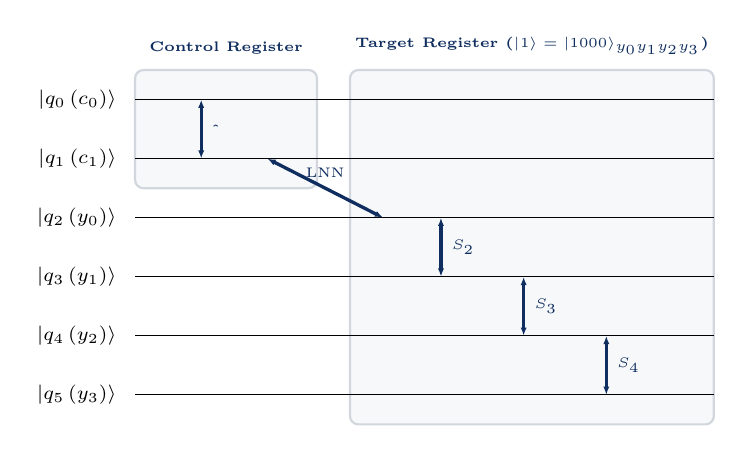
\begin{tikzpicture}[x=1.05cm, y=0.75cm, thick]
    % Register bounding boxes
    \draw[fill=codebg, draw=codeframe, rounded corners=3pt] (-0.3, 3.5) rectangle (1.9, 5.5);
    \node[above=2pt, font=\tiny\bfseries, text=darkblue] at (0.8, 5.5) {Control Register};
    
    \draw[fill=codebg, draw=codeframe, rounded corners=3pt] (2.3, -0.5) rectangle (6.7, 5.5);
    \node[above=2pt, font=\tiny\bfseries, text=darkblue] at (4.5, 5.5) {Target Register ($\ket{1} = \ket{1000}_{y_0 y_1 y_2 y_3}$)};
    
    % Wire lines
    \foreach \y/\l in {5/q_0 \, (c_0), 4/q_1 \, (c_1), 3/q_2 \, (y_0), 2/q_3 \, (y_1), 1/q_4 \, (y_2), 0/q_5 \, (y_3)} {
        \node[left, font=\scriptsize\ttfamily] at (-0.4, \y) {$\ket{\l}$};
        \draw[thin] (-0.3, \y) -- (6.7, \y);
    }
    
    % Nearest neighbor arrows
    \draw[{Latex[length=3pt]}-{Latex[length=3pt]}, darkblue, very thick] (0.5, 5) -- (0.5, 4) node[right, midway, font=\tiny\ttfamily] {\^{}};
    \draw[{Latex[length=3pt]}-{Latex[length=3pt]}, darkblue, very thick] (1.3, 4) -- (2.7, 3) node[above, midway, font=\tiny] {LNN};
    \draw[{Latex[length=3pt]}-{Latex[length=3pt]}, darkblue, very thick] (3.4, 3) -- (3.4, 2) node[right, midway, font=\tiny\ttfamily] {$S_2$};
    \draw[{Latex[length=3pt]}-{Latex[length=3pt]}, darkblue, very thick] (4.4, 2) -- (4.4, 1) node[right, midway, font=\tiny\ttfamily] {$S_3$};
    \draw[{Latex[length=3pt]}-{Latex[length=3pt]}, darkblue, very thick] (5.4, 1) -- (5.4, 0) node[right, midway, font=\tiny\ttfamily] {$S_4$};
\end{tikzpicture}%
}
\caption{Linear Nearest-Neighbor (LNN) spatial tape topology in \texttt{|BF>}, illustrating the adjacent couplings used by the native \texttt{\^{}} primitive. (Profile C control additionally couples the control cell to distant target cells.)}
\label{fig:lnn_tape}
\end{figure}

\subsection{Nearest-Neighbor SWAP Synthesis}
Because distant cells cannot interact directly, any non-local exchange requires a SWAP network. In \texttt{|BF>}, an adjacent SWAP operator $S_k \equiv \text{SWAP}_{k, k+1}$ is expressed as:
\begin{equation}
    S_k = \texttt{\^{}H>H<\^{}>H<H\^{}}
\end{equation}
This sequence executes 3 CNOTs and 4 pointer shifts, leaving pointer position invariant ($\Delta p = 0$).

\subsection{Decomposition of Modular Permutations}

\begin{lemma}[Transposition Decomposition of $U_4$]
On the 4-qubit target register, multiplication by $4 \pmod{15}$ acts as a double transposition:
\begin{equation}
    U_4 \equiv \text{SWAP}(y_0, y_2) \cdot \text{SWAP}(y_1, y_3)
\end{equation}
Compiled to LNN adjacent transpositions, this evaluates to:
\begin{equation}
    U_4 = (S_2 S_3 S_2) \cdot (S_3 S_4 S_3)
\end{equation}
\end{lemma}

\begin{proof}
Under modulo 15 multiplication by 4, the cyclic subgroup pairs exchange as: $1 \leftrightarrow 4$ and $7 \leftrightarrow 13$. In the LSB-first tape basis $\ket{y_0 y_1 y_2 y_3}$:
\begin{align*}
    \ket{1} = \ket{1000} &\leftrightarrow \ket{4} = \ket{0010} \; (\text{transposes } y_0 \leftrightarrow y_2) \\
    \ket{7} = \ket{1110} &\leftrightarrow \ket{13} = \ket{1011} \; (\text{transposes } y_1 \leftrightarrow y_3)
\end{align*}
Since $y_1 = y_3 = 0$ on $\{\ket{1}, \ket{4}\}$ and $y_0 = y_2 = 1$ on $\{\ket{7}, \ket{13}\}$, applying both transpositions independently preserves the invariant subspace. More generally, because $16 \equiv 1 \pmod{15}$, multiplication by $4 = 2^2$ is a cyclic rotation of the 4-bit word by two positions, so the identity holds on all inputs $y \in \{0, \dots, 14\}$ (and fixes $y = 15$). Over an LNN chain, swapping sites $j$ and $j+2$ decomposes into $S_j S_{j+1} S_j$. Thus, $\text{SWAP}(y_0, y_2) = S_2 S_3 S_2$ and $\text{SWAP}(y_1, y_3) = S_3 S_4 S_3$.
\end{proof}

\begin{lemma}[Cyclic Shift Decomposition of $U_7$]
On inputs $y \in \{1, \dots, 14\}$ (in particular on the orbit $\{1, 7, 4, 13\}$), multiplication by $7 \pmod{15}$ is equivalent to a sequential nearest-neighbor swap cascade followed by bit inversion:
\begin{equation}
    U_7 = (X_2 \otimes X_3 \otimes X_4 \otimes X_5) \cdot S_4 \cdot S_3 \cdot S_2
\end{equation}
executed left-to-right on the tape as $S_2$, then $S_3$, then $S_4$, followed by $X^{\otimes 4}$.
\end{lemma}

\begin{proof}
Tracing basis elements in $\ket{y_0 y_1 y_2 y_3}$ under sequential application of $S_2$, $S_3$, $S_4$, and $X^{\otimes 4}$:
$\ket{1} = \ket{1000} \xrightarrow{S_2 S_3 S_4} \ket{0001} \xrightarrow{X^{\otimes 4}} \ket{1110} = \ket{7}$;
$\ket{7} = \ket{1110} \xrightarrow{S_2 S_3 S_4} \ket{1101} \xrightarrow{X^{\otimes 4}} \ket{0010} = \ket{4}$;
$\ket{4} = \ket{0010} \xrightarrow{S_2 S_3 S_4} \ket{0100} \xrightarrow{X^{\otimes 4}} \ket{1011} = \ket{13}$;
$\ket{13} = \ket{1011} \xrightarrow{S_2 S_3 S_4} \ket{0111} \xrightarrow{X^{\otimes 4}} \ket{1000} = \ket{1}$.
The permutation cycle $1 \to 7 \to 4 \to 13 \to 1$ is satisfied exactly, and all three SWAPs ($S_2, S_3, S_4$) act strictly on physical nearest neighbors. In general, $7y \equiv -8y \pmod{15}$: multiplication by $8$ is a one-position cyclic rotation of the 4-bit word, and $15 - z$ is bitwise inversion, which proves the identity for every $y \in \{1, \dots, 14\}$. (Outside this domain the circuit maps $\ket{0} \leftrightarrow \ket{15}$, which is irrelevant here because the target never leaves the orbit of $\ket{1}$.)
\end{proof}

\begin{figure*}[t]
\centering
\resizebox{0.96\textwidth}{!}{%
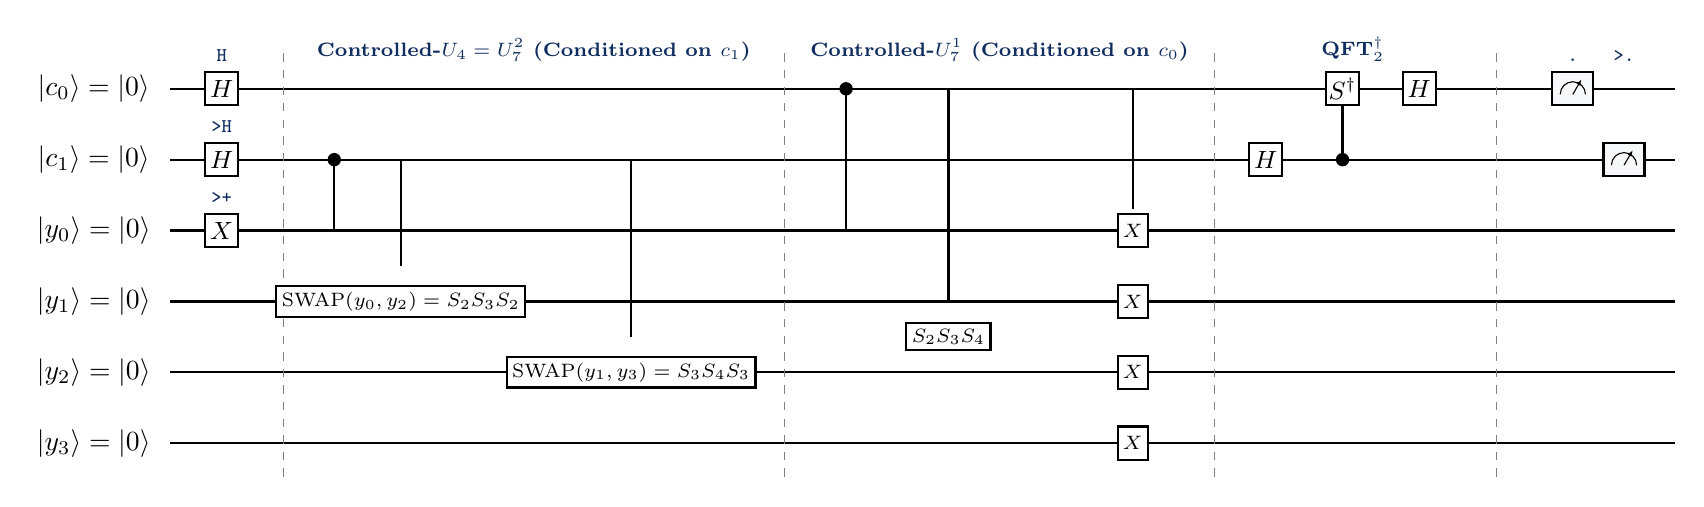
\begin{tikzpicture}[x=0.65cm, y=0.9cm, thick]
    % Wires
    \node at (-1.5, 5) {$\ket{c_0} = \ket{0}$};
    \node at (-1.5, 4) {$\ket{c_1} = \ket{0}$};
    \node at (-1.5, 3) {$\ket{y_0} = \ket{0}$};
    \node at (-1.5, 2) {$\ket{y_1} = \ket{0}$};
    \node at (-1.5, 1) {$\ket{y_2} = \ket{0}$};
    \node at (-1.5, 0) {$\ket{y_3} = \ket{0}$};
    
    \foreach \y in {0,1,2,3,4,5} {
        \draw (0, \y) -- (29.4, \y);
    }
    
    % Stage 1: Init
    \node[above=6pt, font=\scriptsize\ttfamily, text=darkblue] at (1.0, 5) {H};
    \node[gate] at (1.0, 5) {$H$};
    
    \node[above=6pt, font=\scriptsize\ttfamily, text=darkblue] at (1.0, 4) {>H};
    \node[gate] at (1.0, 4) {$H$};
    
    \node[above=6pt, font=\scriptsize\ttfamily, text=darkblue] at (1.0, 3) {>+};
    \node[gate] at (1.0, 3) {$X$};
    
    \draw[dashed, thin, gray] (2.2, 5.5) -- (2.2, -0.5);
    
    % Stage 2: Controlled-U4
    \node[above=6pt, font=\scriptsize\bfseries, text=darkblue] at (7.1, 5) {Controlled-$U_4 = U_7^2$ (Conditioned on $c_1$)};
    \node[control] at (3.2, 4) {};
    \draw[thick] (3.2, 4) -- (3.2, 3);
    \node[draw, fill=white, inner sep=2pt, font=\scriptsize] at (4.5, 2) {$\text{SWAP}(y_0, y_2) = S_2 S_3 S_2$};
    \node[draw, fill=white, inner sep=2pt, font=\scriptsize] at (9.0, 1) {$\text{SWAP}(y_1, y_3) = S_3 S_4 S_3$};
    \draw[thick] (3.2, 4) -| (4.5, 2.5);
    \draw[thick] (3.2, 4) -| (9.0, 1.5);
    
    \draw[dashed, thin, gray] (12.0, 5.5) -- (12.0, -0.5);
    
    % Stage 3: Controlled-U7
    \node[above=6pt, font=\scriptsize\bfseries, text=darkblue] at (16.2, 5) {Controlled-$U_7^1$ (Conditioned on $c_0$)};
    \node[control] at (13.2, 5) {};
    \draw[thick] (13.2, 5) -- (13.2, 3);
    \node[draw, fill=white, inner sep=2pt, font=\scriptsize] at (15.2, 1.5) {$S_2 S_3 S_4$};
    \draw[thick] (13.2, 5) -| (15.2, 2.0);
    
    \node[smallgate] at (18.8, 3) {$X$};
    \node[smallgate] at (18.8, 2) {$X$};
    \node[smallgate] at (18.8, 1) {$X$};
    \node[smallgate] at (18.8, 0) {$X$};
    \draw[thick] (13.2, 5) -| (18.8, 3.3);
    
    \draw[dashed, thin, gray] (20.4, 5.5) -- (20.4, -0.5);
    
    % Stage 4: QFT dagger
    \node[above=6pt, font=\scriptsize\bfseries, text=darkblue] at (23.1, 5) {$\text{QFT}_2^\dagger$};
    \node[gate] at (21.4, 4) {$H$};
    \node[control] at (22.9, 4) {};
    \draw[thick] (22.9, 4) -- (22.9, 5);
    \node[gate] at (22.9, 5) {$S^\dagger$};
    \node[gate] at (24.4, 5) {$H$};
    
    \draw[dashed, thin, gray] (25.9, 5.5) -- (25.9, -0.5);
    
    % Stage 5: Measure
    \node[above=6pt, font=\scriptsize\ttfamily, text=darkblue] at (27.4, 5) {.};
    \node[meter] at (27.4, 5) {};
    \node[above=6pt, font=\scriptsize\ttfamily, text=darkblue] at (28.4, 5) {>.};
    \node[meter] at (28.4, 4) {};
\end{tikzpicture}%
}
\caption{Compiled quantum circuit representation of Shor's Order-Finding algorithm ($N = 15, a = 7$) on a 6-qubit LNN tape.}
\label{fig:shor_circuit}
\end{figure*}

\section{The Complete Full-Register \texttt{|BF>} Program}

Combining initialization, the controlled modular routines, and the 2-qubit inverse QFT yields Listing 1:

\begin{lstlisting}[caption={Complete \texttt{|BF>} program for Shor's Algorithm ($N = 15, a = 7$).}]
H>H>+<
[
  >^H>H<^>H<H^>^H>H<^>H<H^<^H>H<^>H<H^
  >^H>H<^>H<H^>^H>H<^>H<H^<^H>H<^>H<H^
  <<
]
<
[
  >>^H>H<^>H<H^>^H>H<^>H<H^>^H>H<^>H<H^
  <<+>+>+>+
  <<<<<
]
>H[<-->]<H
.>.
\end{lstlisting}

\subsection{Line-by-Line Tape Verification}
\begin{enumerate}
    \item \textbf{Initialization (\texttt{H>H>+<}):} Pointer begins at $p = 0$. Applies $H$ on $c_0$, shifts to $c_1$ (`\texttt{>}'), applies $H$, shifts to $y_0$ (`\texttt{>}'), applies Pauli-$X$ (`\texttt{+}') to prepare $\ket{1} = \ket{1000}_{y_0 y_1 y_2 y_3}$, and steps left to $c_1$ (`\texttt{<}') at $p = 1$.
    \item \textbf{Controlled-$U_4$ Conditioned on $c_1$:} Enters `\texttt{[}' at $p = 1$. The block steps through $y_0 \leftrightarrow y_2$ via \texttt{>S2>S3<S2} and $y_1 \leftrightarrow y_3$ via \texttt{>S3>S4<S3}, ending with \texttt{<<} to return pointer to $p = 1$. Pointer displacement $\Delta p = 0$; $c_1$ is untouched. Profile C executes Controlled-$U_4$.
    \item \textbf{Controlled-$U_7$ Conditioned on $c_0$:} Operator `\texttt{<}' positions pointer at $c_0$ ($p = 0$). Enters `\texttt{[}'. Executes cyclic shift \texttt{>>S2>S3>S4}, steps back via \texttt{<<}, applies Pauli-$X$ across all four cells via \texttt{+>+>+>+}, and traverses left five cells via \texttt{<<<<<} back to $p = 0$. Profile C executes Controlled-$U_7$.
    \item \textbf{Adjacent Inverse QFT ($\text{QFT}_2^\dagger$):} At $p = 0$, shifts to $c_1$ (`\texttt{>}') and applies $H$. Macro \texttt{[<-->]} implements controlled-$S^\dagger$: conditioned on $c_1 = 1$, moves left to $c_0$, executes $S^\dagger = T^\dagger T^\dagger \equiv \texttt{--}$, and returns right. Steps left to $c_0$ (`\texttt{<}') and applies $H$.
    \item \textbf{Readout (\texttt{.>.}):} Measures $c_0 \to \phi_1$, shifts to $c_1$, and measures $c_1 \to \phi_2$, terminating execution.
\end{enumerate}

\subsection{Statevector Evolution \& Sampling}

Tracing the 64-dimensional composite statevector $\ket{\Psi(t)}$ through execution confirms that all cross-terms interfere constructively into exact basis states:
\begin{equation}
    \ket{\Psi_{\text{final}}} = \frac{1}{2}\sum_{s=0}^3 \ket{s}_{c_0 c_1} \otimes \ket{u_s}_{y_0 y_1 y_2 y_3}
\end{equation}
Sampling the classical stream $\mathcal{C} = (c_0, c_1)$ generates the exact probability distribution in Table \ref{tab:measurement_dist}.

\begin{table}[h!]
\centering
\resizebox{\columnwidth}{!}{%
\begin{tabular}{@{}ccccc@{}}
\toprule
Bitstring $(c_0 c_1)$ & Phase $\phi$ & Probability & Order $r$ & Extracted Factors \\
\midrule
\texttt{0 0} & $0.00_2 = 0$   & $25.0\%$ & Trivial ($s = 0$) & \emph{(Resample)} \\
\texttt{0 1} & $0.01_2 = 1/4$ & $25.0\%$ & $r = 4$ & $\mathbf{3, 5}$ \\
\texttt{1 0} & $0.10_2 = 1/2$ & $25.0\%$ & $r' = 2$ (fails check) $\to 2r' = 4$ & $\mathbf{3, 5}$ (after multiple test) \\
\texttt{1 1} & $0.11_2 = 3/4$ & $25.0\%$ & $r = 4$ & $\mathbf{3, 5}$ \\
\bottomrule
\end{tabular}%
}
\caption{Measurement statistics and factor extraction for $N = 15$ (full register: $c_0$ is the most significant phase bit).}
\label{tab:measurement_dist}
\end{table}
The order is read off directly by continued fractions with probability $\varphi(4)/4 = 50\%$ ($s \in \{1, 3\}$); including the multiple test for $s = 2$, the single-shot success probability of the classical post-processing is $75\%$.

\section{Semiclassical Recycling: 5-Qubit Implementation}

While the full-register approach requires 6 qubits, Kitaev's semiclassical iterative phase estimation (IPE) \cite{kitaev1995quantum,griffiths1996semiclassical,monz2016realization} demonstrates that control qubits can be measured sequentially from least significant bit (LSB) to most significant bit (MSB), allowing a single control qubit to be recycled across iterations.

\subsection{Dynamic Loop Architecture}
In \texttt{|BF>}, semiclassical recycling utilizes the active reset token \texttt{,} and \textbf{Profile D} dynamic loops to implement classical feed-forward corrections:

\begin{lstlisting}[caption={Semiclassical 5-qubit Shor algorithm in \texttt{|BF>}.}]
>+<
H [ >^H>H<^>H<H^>^H>H<^>H<H^<^H>H<^>H<H^ >^H>H<^>H<H^>^H>H<^>H<H^<^H>H<^>H<H^ << ] H .
[ >>>>+<<<< , ]
H >>>> [ <<<<-->>>> , ] <<<<
[ >^H>H<^>H<H^>^H>H<^>H<H^>^H>H<^>H<H^ <<+>+>+>+ <<<< ]
H .
\end{lstlisting}

\subsection{Recycled Operational Flow}
The tape width is strictly compressed to $N = 5$ cells:
\begin{equation}
    \text{Tape}_{\text{recycled}} = \Big[ \underbrace{q_0}_{q_{\text{ctrl}}}, \; \underbrace{q_1}_{y_0}, \; \underbrace{q_2}_{y_1}, \; \underbrace{q_3}_{y_2}, \; \underbrace{q_4}_{y_3} \Big]
\end{equation}
\begin{enumerate}
    \item \textbf{LSB Phase Bit ($\phi_2$):} Target is initialized to $\ket{1} = \ket{1000}$ via \texttt{>+<}. Control cell $q_0$ is placed in $\ket{+}$ via $H$. Controlled-$U_4$ produces the entangled state $\frac{1}{\sqrt{2}}(\ket{0}\ket{1000} + \ket{1}\ket{0010})$. Applying $H$ on $q_0$ and measuring (\texttt{.}) yields the LSB $\phi_2 \in \{0, 1\}$ and collapses the target to $\frac{1}{\sqrt{2}}(\ket{1000} + (-1)^{\phi_2}\ket{0010})$.
    \item \textbf{Zero-Ancilla Feed-Forward Stash:} Observe that after $U_4$, target cell $q_4$ ($y_3$) remains in $\ket{0}$ on both $\ket{1000}$ and $\ket{0010}$ (this holds only because the target starts in $\ket{1}$; it would fail for a general eigenstate input, whose support includes $\ket{13} = \ket{1011}$). Loop \texttt{[ >>>>+<<<< , ]} temporarily stashes $\phi_2$ onto $q_4$ and resets $q_0$ to $\ket{0}$.
    \item \textbf{Pre-Commuted Phase Correction \& MSB ($\phi_1$):} Since diagonal phase gate $S^\dagger_0$ commutes with $\mathcal{C}_0(U_7)$, we apply $H$ on $q_0$ and immediately execute \texttt{>>>> [ <<<<-->>>> , ] <<<<}. If $\phi_2 = 1$, this applies $S^\dagger$ (`\texttt{--}') to $q_0$ and actively resets $q_4 \to \ket{0}$ \emph{prior} to Controlled-$U_7$. Controlled-$U_7$ then executes on the restored target register, followed by $H$ and readout (\texttt{.}) to yield MSB $\phi_1$. The classical transcript is therefore $\mathcal{C} = (\phi_2, \phi_1)$, i.e.\ in the \emph{reverse} bit order of the full-register program.
\end{enumerate}
This reduces spatial tape requirements by $16.7\%$ and eliminates all two-qubit $\text{QFT}$ entangling gates (the only remaining phase correction is a classically controlled single-qubit $S^\dagger$). Furthermore, since $y_1 = y_3 = 0$ on $\ket{1}$ and $U_4$ is applied first, $\text{SWAP}(y_1, y_3)$ in $U_4$ acts trivially and can be omitted, reducing the number of native \texttt{\^{}} tokens from 27 to 18.

\subsection{Input-Aware Simplification and the ``Compiled Shor'' Caveat}
The same argument applies to the full-register program: Controlled-$U_4$ is the first operation acting on the target register, which at that point is exactly $\ket{1} = \ket{1000}$, so $\text{SWAP}(y_1, y_3)$ is the identity on every branch and can be dropped. This yields an equivalent 112-token program (\texttt{examples/shor\_15\_full\_opt.bfk}) whose pre-measurement statevector coincides with that of Listing~1 to machine precision.

We stress the distinction from the ``compiled'' Shor demonstrations criticised by Smolin, Smith and Vargo \cite{smolin2013oversimplifying}. Removing a gate that provably acts on qubits known to be $\ket{0}$ uses only knowledge of the \emph{input} state, which any compiler may exploit. By contrast, replacing Controlled-$U_4$ by the two CNOTs that map $\ket{1} \leftrightarrow \ket{4}$, or truncating the multipliers to the orbit $\{1, 7, 4, 13\}$, presupposes knowledge of the period $r$---the very quantity the algorithm is meant to find---and would make the demonstration vacuous. All \texttt{|BF>} programs in this paper implement $U_4$ and $U_7$ as genuine modular multipliers on the full domain $\{1, \dots, 14\}$ (Lemmas 1 and 2); the only input-aware step is the removal of $\text{SWAP}(y_1, y_3)$ described above.

\begin{table*}[t]
\centering
\resizebox{\textwidth}{!}{%
% AUTO-GENERATED by tools/gen_paper_tables.py -- do not edit by hand.
\begin{tabular}{@{}lcccc@{}}
\toprule
Metric & \texttt{|BF>} (6-Qubit Full) & \texttt{|BF>} (6-Qubit Full, opt.) & \texttt{|BF>} (5-Qubit Recycled) & \texttt{|BF>} (5-Qubit Recycled, opt.) \\
\midrule
Tape Register Width ($N$) & 6 & 6 & 5 & 5 \\
Source Instruction Tokens & 149 & 112 & 169 & 132 \\
Native \texttt{\^{}} tokens & 27 & 18 & 27 & 18 \\
Multi-qubit gates, per-token lowering & 27 \texttt{ccx}, 4 \texttt{cx}, 36 \texttt{ch}, 2 \texttt{ctrl @ tdg} & 18 \texttt{ccx}, 4 \texttt{cx}, 24 \texttt{ch}, 2 \texttt{ctrl @ tdg} & 27 \texttt{ccx}, 4 \texttt{cx}, 36 \texttt{ch} & 18 \texttt{ccx}, 4 \texttt{cx}, 24 \texttt{ch} \\
CNOT-equivalents, per-token lowering & 206 & 140 & 202 & 136 \\
Multi-qubit gates, conjugation-aware lowering & 5 \texttt{ccx}, 26 \texttt{cx}, 1 \texttt{ctrl @ sdg} & 4 \texttt{ccx}, 18 \texttt{cx}, 1 \texttt{ctrl @ sdg} & 5 \texttt{ccx}, 26 \texttt{cx} & 4 \texttt{ccx}, 18 \texttt{cx} \\
CNOT-equivalents, conjugation-aware lowering & \textbf{58} & \textbf{44} & \textbf{56} & \textbf{42} \\
Circuit depth (ASAP), conjugation-aware & 51 & 36 & 50 & 35 \\
Max.\ interaction distance (all-to-all lowering) & 5 & 5 & 4 & 4 \\
\midrule
\multicolumn{5}{@{}l}{\emph{Open linear chain (LNN): exact 1-/2-qubit decomposition + SWAP routing}} \\
Routing SWAPs inserted & 22 & 20 & 21 & 17 \\
CNOT-equivalents incl.\ SWAPs (SWAP $= 3$) & \textbf{124} & \textbf{104} & \textbf{119} & \textbf{93} \\
Circuit depth (ASAP), LNN & 120 & 92 & 121 & 93 \\
Max.\ interaction distance, LNN & 1 & 1 & 1 & 1 \\
Measurements incl.\ loop tests / resets & 2 / 0 & 2 / 0 & 6 / 2 & 6 / 2 \\
\bottomrule
\end{tabular}
%
}
\caption{Resource analysis of the \texttt{|BF>} Shor programs ($N = 15$, $a = 7$), generated automatically from the reference transpiler by \texttt{tools/gen\_paper\_tables.py} (the test suite fails if this table is stale). CNOT-equivalents use standard decompositions: Toffoli $= 6$, controlled-phase ($T$, $T^\dagger$, $S$, $S^\dagger$) $= 2$, \texttt{cx}/\texttt{cz}/\texttt{ch} $= 1$. Per-token lowering controls every token of a Profile C block; conjugation-aware lowering (Sec.~\ref{sec:conj}) controls only the gates that are not undone inside the block. The upper block assumes all-to-all connectivity: there, coherent controls couple $c_0$/$c_1$ (resp.\ $q_0$) to target cells up to five positions away. The lower block gives the cost on an open linear chain after exact decomposition into 1- and 2-qubit gates and SWAP routing (Sec.~\ref{sec:lnn}); every 2-qubit gate then acts on adjacent qubits. Loop-test measurements of the semiclassical programs are included in the measurement count.}
\label{tab:resource_comparison}
\end{table*}

\section{Transpilation to OpenQASM 3.0}

Because pointer arithmetic (\texttt{>}, \texttt{<}) can be computed statically at compile time, pointer movement emits no gates. OpenQASM 3.0 gate modifiers such as \texttt{ctrl @} apply only to named gates (there are no anonymous controlled blocks), so the automatic transpiler lowers every token of a Profile C block to its controlled counterpart (\texttt{\^{}}$\to$\texttt{ccx}, \texttt{H}$\to$\texttt{ch}, \texttt{+}$\to$\texttt{cx}, \dots), assigns one transcript bit per \texttt{.} token, and uses separate \texttt{guard} bits for Profile D loop tests.

\subsection{Conjugation-Aware Lowering of Profile C Blocks}
\label{sec:conj}
Controlling every token of a Profile C block is correct but wasteful. The transpiler instead exploits the elementary identity
\begin{equation}
    \mathcal{C}_p\!\left(V U V^{-1}\right) = V \, \mathcal{C}_p(U) \, V^{-1},
\end{equation}
valid for arbitrary unitaries $U, V$: if the control is $\ket{0}$, $V$ and $V^{-1}$ cancel. A dynamic program over the block's gate list chooses, for every contiguous segment, the cheaper of (i) splitting it into independently controlled parts and (ii) peeling off a prefix $V$ whose inverse forms the matching suffix, leaving $V$ uncontrolled; nested Profile C blocks are lowered first, and adjacent phase gates are merged ($T^\dagger T^\dagger \to S^\dagger$). For the SWAP macro $S_k = \texttt{\^{}}\,(\texttt{H>H<\^{}>H<H})\,\texttt{\^{}}$ this applies twice and gives $\mathcal{C}(S_k) = \text{CNOT}\,(H \otimes H)\,\text{Toffoli}\,(H \otimes H)\,\text{CNOT}$, i.e.\ 8 instead of 22 CNOT-equivalents. It also recognises that a distance-two transposition $S_j S_{j+1} S_j = V S_{j+1} V^{-1}$ with $V = S_j$ needs only its middle SWAP controlled. Together this reduces the 6-qubit program from 206 to 58 CNOT-equivalents (Table~\ref{tab:resource_comparison}). Equivalence of the optimized and per-token lowerings with the abstract machine is checked exactly, by an independent OpenQASM interpreter, on all example programs and on several hundred randomly generated programs (differential fuzzing).

\subsection{Routing onto an Open Linear Chain}
\label{sec:lnn}
To make the nearest-neighbor question measurable rather than rhetorical, the transpiler provides an LNN mode. First, every gate acting on three or more qubits is decomposed \emph{exactly} into 1- and 2-qubit gates: the Toffoli by the standard Clifford+$T$ circuit with six CNOTs \cite{nielsen2010quantum}; multi-controlled phases recursively,
\begin{equation}
\begin{aligned}
    C^{k}P(\varphi) ={} &\mathrm{CP}_{c_k t}(\tfrac{\varphi}{2})\, C^{k-1}X_{c_k}\, \mathrm{CP}_{c_k t}(-\tfrac{\varphi}{2}) \\
    &\cdot C^{k-1}X_{c_k}\, C^{k-1}P(\tfrac{\varphi}{2}),
\end{aligned}
\end{equation}
(written in time order, with $C^{k-1}X_{c_k}$ controlled by $c_1, \dots, c_{k-1}$) together with $C^kX = H\,C^kP(\pi)\,H$, $C^kZ = H\,C^kX\,H$ and $C^kH = R_y(\tfrac{\pi}{4})\,C^kZ\,R_y(-\tfrac{\pi}{4})$ (operator products, i.e.\ $R_y(-\tfrac{\pi}{4})$ is applied first) \cite{barenco1995elementary}. Second, the resulting 2-qubit gates are routed on an open chain: a logical-to-physical layout is tracked and adjacent SWAPs are inserted greedily, choosing which endpoint to move by a short lookahead over the upcoming gates. Bodies of Profile D loops restore the layout they started with, so every iteration sees the same placement. Ring-wrapping \texttt{\^{}} tokens at $p = N-1$ are routed like any other non-adjacent gate.

For the 6-qubit program this yields 22 routing SWAPs and 124 CNOT-equivalents (including SWAPs at 3 CNOTs each), versus 58 with all-to-all connectivity; the optimized 5-qubit recycled program needs 17 SWAPs and 93 CNOT-equivalents (Table~\ref{tab:resource_comparison}). Strict nearest-neighbor execution therefore costs roughly a factor of two over the all-to-all lowering. The router is a simple greedy heuristic, so these figures are upper bounds rather than optima. Exactness of every decomposition and of the routed circuits (including 4-controlled gates) is verified against the abstract machine by the independent interpreter and the differential fuzzer.

Listing~3 gives an equivalent, hand-structured form of Listing~1 that wraps the modular multipliers in named gates:

\begin{lstlisting}[language=C, caption={Hand-structured OpenQASM 3.0 circuit equivalent to the full-register \texttt{|BF>} Shor program.}]
OPENQASM 3.0;
include "stdgates.inc";

// Modular multiplication by 4 (SWAP network on y0..y3)
gate u4 y0, y1, y2, y3 {
    // Transposition (y0, y2)
    cx y0, y1; h y0; h y1; cx y0, y1; h y1; h y0; cx y0, y1;
    cx y1, y2; h y1; h y2; cx y1, y2; h y2; h y1; cx y1, y2;
    cx y0, y1; h y0; h y1; cx y0, y1; h y1; h y0; cx y0, y1;
    // Transposition (y1, y3)
    cx y1, y2; h y1; h y2; cx y1, y2; h y2; h y1; cx y1, y2;
    cx y2, y3; h y2; h y3; cx y2, y3; h y3; h y2; cx y2, y3;
    cx y1, y2; h y1; h y2; cx y1, y2; h y2; h y1; cx y1, y2;
}

// Modular multiplication by 7 (SWAP cascade + bit inversion)
gate u7 y0, y1, y2, y3 {
    cx y0, y1; h y0; h y1; cx y0, y1; h y1; h y0; cx y0, y1;
    cx y1, y2; h y1; h y2; cx y1, y2; h y2; h y1; cx y1, y2;
    cx y2, y3; h y2; h y3; cx y2, y3; h y3; h y2; cx y2, y3;
    x y0; x y1; x y2; x y3;
}

qubit[6] q;
bit[2] c;

// Initialization
h q[0];
h q[1];
x q[2];

ctrl @ u4 q[1], q[2], q[3], q[4], q[5];   // Controlled-U4 on c1
ctrl @ u7 q[0], q[2], q[3], q[4], q[5];   // Controlled-U7 on c0

// 2-Qubit Inverse QFT on (q[0], q[1]) without final SWAP
h q[1];
ctrl @ tdg q[1], q[0];
ctrl @ tdg q[1], q[0];
h q[0];

// Computational basis readout: c[0] = phi_1 (MSB), c[1] = phi_2 (LSB)
c[0] = measure q[0];
c[1] = measure q[1];
\end{lstlisting}

\section{NISQ Fidelity Estimate}

On physical quantum hardware characterized by single-qubit error rate $\epsilon_1 \approx 10^{-4}$, two-qubit CNOT gate error $\epsilon_2 \approx 5 \times 10^{-3}$, and transverse dephasing time $T_2$, circuit survival fidelity is commonly modelled as:
\begin{equation}
    \mathcal{F} \approx (1 - \epsilon_1)^{G_1} (1 - \epsilon_2)^{G_2} \exp\!\left(-\frac{D \cdot \tau_g}{T_2}\right)
\end{equation}
Counting only the two-qubit factor with the CNOT-equivalents of Table~\ref{tab:resource_comparison}, the per-token lowering of the 6-qubit program ($G_2 = 206$) gives $(1-\epsilon_2)^{206} \approx 0.36$, whereas the conjugation-aware lowering ($G_2 = 58$) gives $\approx 0.75$; the input-simplified 6-qubit program ($G_2 = 44$) and the optimized 5-qubit recycled program ($G_2 = 42$) reach $\approx 0.80$ and $\approx 0.81$ with all-to-all connectivity. On a strict open chain the routed circuits ($G_2 = 124$ and $93$) give $\approx 0.54$ and $\approx 0.63$, respectively (decoherence not included). The dominant cost is the coherent control of the SWAP networks, not the native \texttt{\^{}} primitive itself, which is why control-aware lowering matters more than any other optimization considered here.

\section{Conclusion \& Future Work}

We have demonstrated that Shor's algorithm for $N = 15$, $a = 7$ can be compiled into the minimal \texttt{|BF>} calculus, with the modular multipliers expressed as nearest-neighbor SWAP networks and an exact phase readout, and that semiclassical dynamic loops reduce the register to five qubits without two-qubit QFT gates. The coherent control of these networks is not nearest-neighbor and dominates the gate cost after lowering; conjugation-aware lowering reduces it by a factor of about 3.5 (206 $\to$ 58 CNOT-equivalents for the 6-qubit program). Routed exactly onto an open linear chain, the programs remain executable with roughly twice the all-to-all cost. Future work will replace the greedy router by optimal SWAP placement, exploit relative-phase Toffolis where phases cancel, extend this framework to general modular exponentiation using linear reversible carry-ripple adders \cite{fowler2004lnn,beauregard2003circuit}, and pursue formal verification of the lowering within mechanized proof assistants.

\begin{thebibliography}{99}

\bibitem{shor1994algorithms}
P.~W. Shor, ``Algorithms for quantum computation: discrete logarithms and factoring,'' in \emph{Proc. 35th Ann. Symp. on Foundations of Computer Science (FOCS '94)}, pp.~124--134, IEEE, 1994, \href{https://doi.org/10.1109/SFCS.1994.365700}{doi:10.1109/SFCS.1994.365700}.

\bibitem{shor1999polynomial}
P.~W. Shor, ``Polynomial-time algorithms for prime factorization and discrete logarithms on a quantum computer,'' \emph{SIAM Review}, vol.~41, no.~2, pp.~303--332, 1999, \href{https://doi.org/10.1137/S0036144598347011}{doi:10.1137/S0036144598347011}.

\bibitem{matocl2026bf}
mat-ocl, ``\texttt{|BF>} (Bra-Ket-Fuck): A Vacuum-Initialized Clifford+$T$ Quantum Tape Architecture for Linear Nearest-Neighbor Compilation and Formal Verification,'' \emph{Technical Whitepaper v1.0}, Systems \& Quantum Esoteric Architecture Working Group, Oct. 2026.

\bibitem{muller1993brainfuck}
U.~M{\"u}ller, ``Brainfuck,'' 1993, \href{https://en.wikipedia.org/wiki/Brainfuck}{online archive}.

\bibitem{dirac1939notation}
P.~A.~M. Dirac, ``A new notation for quantum mechanics,'' \emph{Math. Proc. Cambridge Philos. Soc.}, vol.~35, no.~3, pp.~416--418, 1939, \href{https://doi.org/10.1017/S0305004100021162}{doi:10.1017/S0305004100021162}.

\bibitem{nielsen2010quantum}
M.~A. Nielsen and I.~L. Chuang, \emph{Quantum Computation and Quantum Information}, 10th Anniversary ed., Cambridge University Press, 2010, \href{https://doi.org/10.1017/CBO9780511976667}{doi:10.1017/CBO9780511976667}.

\bibitem{fowler2004lnn}
A.~G. Fowler, S.~J. Devitt, and L.~C.~L. Hollenberg, ``Implementation of Shor's algorithm on a linear nearest neighbour qubit array,'' \emph{Quantum Info. Comput.}, vol.~4, no.~4, pp.~237--251, 2004, arXiv:\href{https://arxiv.org/abs/quant-ph/0402196}{quant-ph/0402196}.

\bibitem{saeedi2011lnn}
M.~Saeedi, R.~Wille, and R.~Drechsler, ``Synthesis of quantum circuits for linear nearest neighbor architectures,'' \emph{Quantum Information Processing}, vol.~10, no.~3, pp.~355--377, 2011, \href{https://doi.org/10.1007/s11128-010-0201-2}{doi:10.1007/s11128-010-0201-2}.

\bibitem{kitaev1995quantum}
A.~Y. Kitaev, ``Quantum measurements and the Abelian Stabilizer Problem,'' 1995, arXiv:\href{https://arxiv.org/abs/quant-ph/9511026}{quant-ph/9511026}.

\bibitem{griffiths1996semiclassical}
R.~B. Griffiths and C.-S. Niu, ``Semiclassical Fourier transform for quantum computation,'' \emph{Phys. Rev. Lett.}, vol.~76, no.~17, pp.~3228--3231, 1996, \href{https://doi.org/10.1103/PhysRevLett.76.3228}{doi:10.1103/PhysRevLett.76.3228}.

\bibitem{barenco1995elementary}
A.~Barenco, C.~H. Bennett, R.~Cleve, D.~P. DiVincenzo, N.~Margolus, P.~Shor, T.~Sleator, J.~A. Smolin, and H.~Weinfurter, ``Elementary gates for quantum computation,'' \emph{Phys. Rev. A}, vol.~52, no.~5, pp.~3457--3467, 1995, \href{https://doi.org/10.1103/PhysRevA.52.3457}{doi:10.1103/PhysRevA.52.3457}.

\bibitem{monz2016realization}
T.~Monz, D.~Nigg, E.~A. Martinez, M.~F. Brandl, P.~Schindler, R.~Rines, S.~X. Wang, I.~L. Chuang, and R.~Blatt, ``Realization of a scalable Shor algorithm,'' \emph{Science}, vol.~351, no.~6277, pp.~1068--1070, 2016, \href{https://doi.org/10.1126/science.aad9480}{doi:10.1126/science.aad9480}.

\bibitem{smolin2013oversimplifying}
J.~A. Smolin, G.~Smith, and A.~Vargo, ``Oversimplifying quantum factoring,'' \emph{Nature}, vol.~499, no.~7457, pp.~163--165, 2013, \href{https://doi.org/10.1038/nature12290}{doi:10.1038/nature12290}.

\bibitem{beauregard2003circuit}
S.~Beauregard, ``Circuit for Shor's algorithm using $2n+3$ qubits,'' \emph{Quantum Info. Comput.}, vol.~3, no.~2, pp.~175--185, 2003, arXiv:\href{https://arxiv.org/abs/quant-ph/0205095}{quant-ph/0205095}.

\end{thebibliography}

\end{document}
